\section{Sistemas de V�deo \label{sistemas_de_video}}

teste Os sistemas de v�deo consistem na organiza��o em que uma determinada
informa��o de v�deo � armazenada em forma digital, tais como AVI,
MPEG, entre outros. O MPEG (Movie Pictures Experts Group) � um
padr�o internacional definido pela ISO que tem como caracter�stica a
compress�o de um v�deo. Onde ao comprimir uma determinada amostragem
de um v�deo, o mesmo � passado pelo canal compressor, e ao exibir
esta mesma amostragem o v�deo passa pelo canal expansor.

\begin{figure}[h|top]
 \centering
 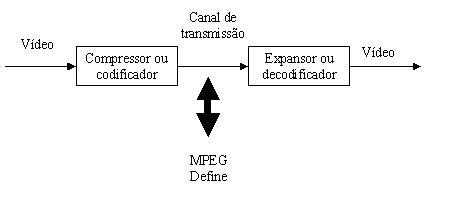
\includegraphics[width=0.7\linewidth]{imagens/mpeg.png}
 \caption{Sistema de Codifica��o e Decodifica��o de um v�deo no formato MPEG.}
 \label{img_mpeg}
\end{figure}


\begin{figure}[h|top]
 \centering
 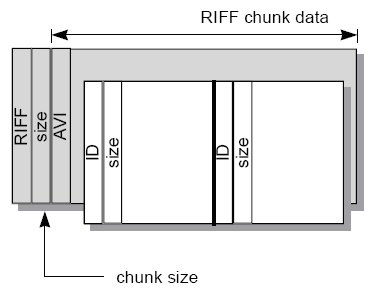
\includegraphics[width=0.7\linewidth]{imagens/avi.png}
 \caption{Sistema de armazenamento AVI.}
 \label{img_avi}
\end{figure}

O AVI (Audio Video Interleave) � um padr�o criado pela Microsoft em
1992, o qual � derivado do padr�o RIFF que divide os dados em
blocos. Ao contr�rio dos outros padr�es o AVI n�o possui compress�o.
